%**************************************************
%			SDN-OpenFlow.tex
%**************************************************
\section{SDN and OpenFlow overview}
\frame
{
\frametitle{SDN and OpenFlow overview}
\tableofcontents[currentsection]
\addtocounter{framenumber}{-1}
}

\begin{frame}{SDN Overview \small{1/3}}
SDN architecture is composed by:
\begin{figure}
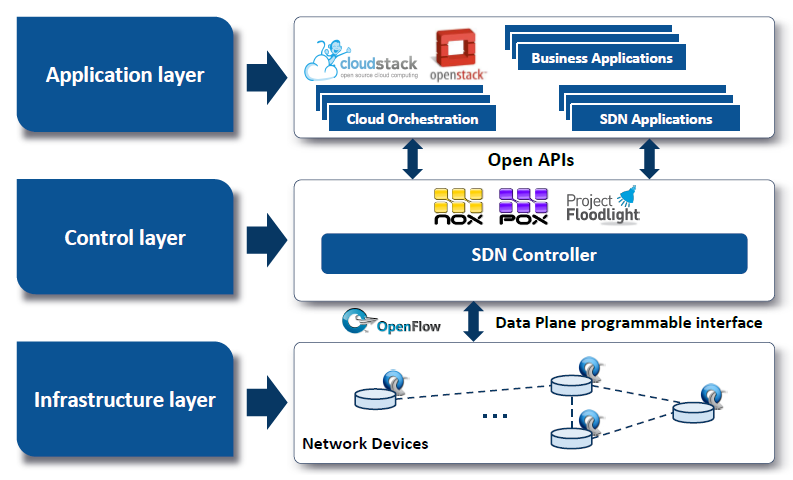
\includegraphics[scale=0.45]{Immagini/SDNStructure.png}
\caption{SDN architecture}
\label{fig:SDN-architecture}
\end{figure}
\end{frame}

\begin{frame}{OpenFlow switch Overview \small{2/3}}
\begin{figure}
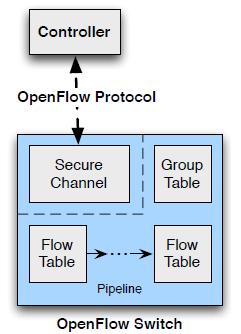
\includegraphics[scale=0.45]{Immagini/OpenFlowSwitch.png}
\caption{OpenFlow switch}
\label{fig:OpenFlowSwitchComponent}
\end{figure}
\end{frame}

\begin{frame}{OpenFlow switch pipeline \small{3/3}}
\begin{figure}
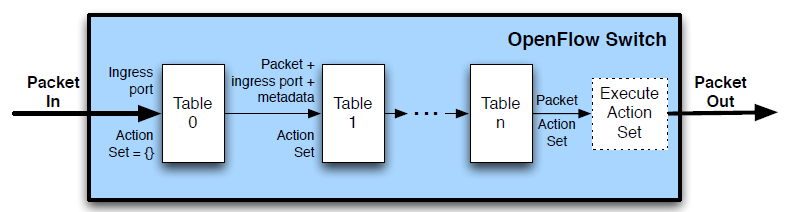
\includegraphics[scale=0.45]{Immagini/OpenFlowPipeline.png}
\caption{OpenFlow switch pipeline}
\label{fig:OpenFlowSwitchPipeline}
\end{figure}
\end{frame}

\subsection{Benefits}
\begin{frame}{Benefits}
Using SDN with OpenFlow in network management there are benefits, like:
\begin{itemize}
\item<2-> centralized control of routers/switches multi vendor
\item<3-> reduction of complexity through automation
\item<4-> an high rate of innovation
\item<5-> high level of reliability and a more granular level of control of entire network
\end{itemize}
\end{frame}